\documentclass[uplatex, dvipdfmx]{article}
\usepackage{amsmath, amsthm, amssymb}
\usepackage{ascmac,here,txfonts,txfonts}
\usepackage[margin=2.5cm]{geometry}
\usepackage{color}
\usepackage{graphicx}
\usepackage{algorithm}
\usepackage{algorithmic}
\usepackage[subrefformat=parens]{subcaption}
\usepackage{hyperref}
\usepackage{csquotes}
\usepackage[backend=biber, style=numeric, sorting=none]{biblatex}
\usepackage[format=hang]{caption}
\usepackage[format=hang, subrefformat=parens]{subcaption}

\captionsetup{compatibility=false}

\addbibresource{../references.bib}

\setlength{\parindent}{0.3in}

\title{ Iterated Inversion System: An Efficient Algorithm to Visualize Kleinian Groups Based on Inversions }
\author{ Kento Nakamura\\
Meiji University\\
}

\date{}

\pagestyle{headings}

\begin{document}

\maketitle

\begin{abstract}
 Kleinian group is one of the fields of mathematics. Visualized
 Kleinian group shows us beautiful fractal structure, and clues to
 understand their mathematical properties.
 However, it often takes much time to render Kleinian group.
 Thus, we invent an efficient algorithm to visualize Kleinian groups. 
 The algorithm is called Iterated Inversion System
 (IIS.) It can render not only two dimensional objects but also three
 dimensional objects.
 We summarize the usage of the IIS and its applications.
\end{abstract}

\clearpage

\tableofcontents

\clearpage

\section*{Acknowledgement}
This is acknowledgement

%#!uplatex main.tex

\section{Introduction}

In this paper, we introduce efficient algorithm to visualize Kleinian
groups.
Kleinian group theory is one of the fields of mathematics studying 
M\"obius transformation groups.
It is well suited to visualization and computer experiment.

%% 並列計算によって高速な描画が可能になった

In this paper, we introduce basic usage of the IIS algorithm and its
applications.

%% クライン群論は可視化と相性がよく,コンピュータによる計算実験や可視化
%% によって研究が進んだ一側面もある.可視化には様々な方法があるが,基本
%% 的に時間がかかる.
%% 我々は,一部のクライン群を直観的かつ高速に描画することを可能にするア
%% ルゴリズム,Iterated Inversion Systemを開発した.
%% この論文では,そのアルゴリズムの概要と応用範囲を記述する


%#BIBTEX biber --bblencoding=utf8 -u -U --output_safechars main
%#!uplatex main.tex

\section{Preparation}

In this section, we introduce some mathematical terms and prerequisites
to understand the IIS algorithm and basic usage of IIS.

\subsection{Terminology}

In this paper, we use terms about Kleinian groups used in Indra's
Pearls \cite{MumfordSeriesWright200204}.
The word \textit{group} represents an algebraic group which is
central concept about group theory.
Algebraic group is a set which has multiplication and identity element, satysfies associative law, and whose each element of the group has inverse element.
% Algebraic group is a set which has multiplication, satysfies the associative law, has a unit, and has an inverse element for each element.

Also, a transformation group is an algebraic group consists of transformations about plane or space.
However, in this case, because we assume M\"obius transformation group, we add infinity $\infty$ to complex plane $\mathbb{C}$ (or three
dimensional space $\mathbb{R}^3$) and apply one-point compactification to the set.
We consider a group composed of the element of homeomorphic mapping on
the set $\tilde{ \mathbb{C}}$ (or $\tilde{ \mathbb{R}^3 }$.)
%Here we consider the plane or the space with the infinity $\infty$.  That is, we consider the one-point compactification of
%$\mathbb{C}$ and it is denoted by $\tilde{\mathbb{C}}$.  In the same way, the one-point compactification of $\mathbb{R}^3$ is 
%denoted by $\tilde{ \mathbb{R}^3 }$.
%The two dimensional M\"obius transformation group $\mathrm{M\"ob}(\tilde{\mathbb{C}})$ is the set of M\"obius transfromation. 
%The definition of a M\"obius transformation will be introduced later. 
%This is a group with respect to the composite of transormations.  The unit is the identity map and the inverse element is the 
%inverse transformation.  In the same manner, we consider the three dimensional M\"obius transformation group $\mathrm{M\"ob}(\tilde{\mathbb{R}}^3)$
%説明の順番として、まず空間を説明して、そののちに写像を説明する。

We assume that transformations $f(z)$ and $g(z)$ are complex functions
whose parameter is complex number $z$
and homeomorphic mappings on $\hat{\mathbb{C}}$.
What transformation group $G$ is generated by $f(z)$,$g(z)$
is any element of $G$ are represented by some composite mappings of $f(z)$,
$g(z)$, $f^{-1}(z)$, and $g^{-1}(z)$
%2元生成のメビウス変換群についての記述はこのあと見られないので、この説明は省けるのではないか。

In this paper, for simplicity, we use
lower case alphabets such as $a$ and $b$ instead of $f(z)$ and $g(z)$ and
upper case alphabet such as $A$ and $B$ instead of $f^{-1}(z)$ and $g^{-1}(z)$
%メビウス変換をa,b,A,Bで表すような記述はこのあと見られないので、この説明は省けるのではないか。

From this point, we assume transformation group $G$ is generated by two
elements $a$ and $b$. Arbitrary elements of $G$ is represented by
four alphabet $a$, $b$, $A$, and $B$ and we follow the rule of inverse
 of $a$ is $A$ and inverse of $b$ is $B$.
Thus, composite mapping $f(z)\circ g(z) \circ f^{-1}(z)$ simply
is represented by $abA$.
%上で、「変換群は合成を演算とする」と書いてあるので、改めて説明する必要もなくなった。
%このあたりの説明は、あとあとに生成元の無限巡回によるリミットポイントの説明が出てくるのかどうか、に依存している。
%極限集合を説明するところに移動してはどうか。

Following the rule of the words, we represent circular infinite words as
bar, that is, $aaaa\cdots$ is represented by $\overline{a}$ and $abABabAB \cdots$ 
is represented by $\overline{abAB}$.
These infinite words are not element of $G$. However, when we consider
the orbit by $G$, we use such notations to express the limit set.
%このあたりの説明は、あとあとに生成元の無限巡回によるリミットポイントの説明が出てくるのかどうか、に依存している。
%極限集合を説明するところに移動してはどうか。

\subsection{Inversions in Circles or Spheres}

It is known that M\"obius transformations on $\tilde{\mathbb{C}}$
are composed of even number of inversions in circles.
Here, it is assumed that the inverse mapping about circle centered at
$C\in\mathbb{C}$ and radius $R\in\mathbb{R}$ ($R>0$).
The formula is given by
$f(z) = \frac{R^2}{~\overline{z -C}~} + C$.
According to the definition, inverse mapping is a homeomorphic mapping on
$\tilde{\mathbb{C}}$.

In this context, the circles do not center infinity, but 
by interpreting the line on complex plane as ``the circle whose center is
infinitely far point and radius is infinity'', 
line symmetry transformation (but infinitely far point is
transformed to infinitely far point) on complex plane 
is also inversion in the circle.
Inversion mapping (including line symmetry transformation) does not
preserve direction of complex plane.
Thus compositions of even number of inversion mapping are homeomorphic
mappings preserving direction of complex plane.

Later, we compute Jacobian of inverse mapping.
This is Jacobian matrix as mapping from complex plane to complex plane.
Generally, inverse mapping preserve angles.
From this property, Jacobian mapping is given by multiplication of complex
number.
Concretely, Jacobian is composed of rotations and constant scaling
and absolute value of Jacobian is as follows
$Jacobian = R^2 / distance(P,~C)^2$
where $P$ is a point before applying the inversion.

In the similar manner to circle inversions we can determine inversion
mapping about spherical surface $S^2$ included in $\tilde{\mathbb{R}^3}$.
Here, image of the inversion mapping is determined by center of the sphere and
distance to the center.
Concretely, $f(z) = \frac{R^2}{~\overline{z -C}~} + C$.
Also, a plane $\alpha$ included in $\mathbb{R}^3$ is considered as
sphere whose center and radius are infinity.
In this case, the inversion mapping about the plane $\alpha$ is plane symmetry
transformation about $\alpha$.

\subsection{M\"obius Transformations}

In this study, we handle actions on $PSL_2\mathbb{C}$ of $\hat{\mathbb{C}}$.
M\"obius transformation is defined on $\hat{\mathbb{C}}$ and
linear fractional transformation
$f(z)=\dfrac{az+b}{cz+d}$ for complex variable $z$ where constants
$a, b, c, d$ are complex number and satisfy $ad - bc = 1$.
Such linear fractional transformation $f(z)$ is conformal homeomorphic
mapping and preserves direction of $\hat{\mathbb{C}}$.

As a group acting on $\hat{\mathbb{C}}$, a set of linear fractional
transformation $f(z) = \dfrac{az + b}{cz + d}$
and a set of $2 \times 2$ matrix
$\begin{pmatrix}a & b \\ c& d \end{pmatrix}$
$PSL_2\mathbb{C}$ are same type.
So, in this place, we use linear fractional transformation and
complex two-dimensional projective special linear group
$PSL_2\mathbb{C}$ without distinction.

Also it is known that any M\"obius transformation can be represented by
even number of circle inversions.
The compositions of M\"obius transformations is also M\"obius
transformations. A set of all of the M\"obius transformations makes
groups. For more details about M\"obius transformation, refer
\cite{MumfordSeriesWright200204}\cite{marden_2016}.

For a group $G$, mapping $G \times X \to X$ is actions of a group
satisfying following conditions.
\begin{enumerate}
 \item e $\cdot$ x = x for all x in X. (Here, e denotes the identity element of
       the group G.)
 \item (gh) $\cdot$ x = g $\cdot$ (h$\cdot$ x) for all g, h in G and all x in X.
       (Here, gh denotes the result of applying the group operation of G to the elements g and h.)
\end{enumerate}
This is also called group $G$ acts on space $X$.
In this sense, a set of the linear fractional transformations acts on
$\hat{\mathbb{C}}$

When all of the constant numbers of M\"obius transformations are real number,
that is, $a, b, c, d \in \mathbb{R}$, $f(z)$ preserve upper-half plane.
Moreover, Metric of upper-half plane preserves
$\dfrac{ds^2}{(\mathrm{Im}z)}$
Thus, a set of linear fractional transformations whose all of constants
are real number acts on hyperbolic plane as isometric transformation group.

When the constants $a, b, c, d$ are complex number, it is thought that
$f(z)$ acts on hyperbolic space.
As the model of hyperbolic space $mathbb{H}^3$, we consider upper half
space model, but we consider three-dimensional space as the coordinates
$(z, t)$, and $z$ is complex coordinates and $t$ is real coordinates.
Upper-half space model is a model of hyperbolic space whose universal
set is $\{(z,t) \mid t>0\}\cup \{ \infty \}$.
$\hat{\mathbb{C}} = \{ (z,0) \mid z \in \mathbb{C}\} \cup \{ \infty\}$
is its set of infinitely far points. M\"obius transformations are groups acting on
the set of infinitely far points. However, it is known that by Poincare
expansion, M\"obius transformations are extended to isometric mapping
in hyperbolic space.
For the relationship between M\"obius transformations and hyperbolic
space, refer 
\cite{Marden200705outerCircles}\cite{taniguchi_okumura199610invitation}

From the above, researching M\"obius transformation groups is heavily
related to studying three-dimensional hyperbolic geometry and hyperbolic
polyhedra.

Also, in this paper, we also use a concept extending a M\"obius
transformation to a $\mathbb{R}^3\cup\{\infty\}$.
Concretely, we define composition of even number of inversion mapping
about a sphere as a three-dimensional M\"obius transformation.
The definition is extended relation between inversions in a circle and
M\"obius transformation.
In that sense, M\"obius transformation should be called two-dimensional
M\"obius transformation, but
simply they are called differently M\"obius transformation and
three-dimensional M\"obius transformation without confusion.

Three-dimensional M\"obius transformations are deeply related to
four-dimantional hyperbolic space. Actually, we assume four-dimensional
hyperbolic upper half space model, its infinite far point set is
$\mathbb{R}^3\cup\{\infty\}$, and it is known that three-dimensional M\"obius
transformation gives orientation preserving isometric transformation in
four-dimensional hyperbolic space via poincare expansion.
In this sense studying three-dimensional M\"obius transformation is
deeply related to four-dimensional hyperbolic space or four-dimensional
hyperbolic space and four-dimensional hyperbolic polyhedra.
To represent three-dimensional M\"obius transformation using matrix
there are Quaternion matrix sub-group of $2 \times 2$ matrix called
$Sp^k(1,1)$. About this topic, refer
\cite{sakugawa2010limit}\cite{sakugawa2007master}.


\subsection{Classification of M\"obius Transformations}

Excluding the identical mapping, M\"obius transformations
$f(z) = \dfrac{az + b}{cz + d}$ are classified as three types.
They are \textit{Elliptic}, \textit{Parabolic}, and \textit{Loxodromic}.
By the knowledge of linear algebra, the standard form of $PSL_2\mathbb{C}$
is either one of $\begin{pmatrix}1 & a \\ 0 & 1 \end{pmatrix}$ or
$\begin{pmatrix}\lambda & 0 \\ 0 & \lambda^{-1} \end{pmatrix}$.
The former one of $f(z)$ is parabolic transformations.
For parabolic transformation the number of fixed point is one, and
$2 \times 2$ square matrix $X$ satisfy $\mathrm{tr}^2X = 4$

When the standard form is
$\begin{pmatrix}\lambda & 0 \\ 0 & \lambda^{-1} \end{pmatrix}$
or absolute value of lambda is one, that is  $|\lambda|$ is $1$, 
$f(z)$ is called elliptic transformations.
The properties of elliptic transformation are they have
two fixed points and the transformation gives rotations around fixed
points.
Also, the matrix representation $\mathrm{tr}^2X > 4$ is 
necessary and sufficient conditions.
In addition, the m\"obius transformation having finite order
is elliptic transformation.

When the standard form is
$\begin{pmatrix}\lambda & 0 \\ 0 & \lambda^{-1} \end{pmatrix}$
and complex number $|\lambda| \neq 1$, $f(z)$ is called loxodromic.
If $\lambda$ is real number exclude in $1$, the transformation is called
\textit{hyperbolic} too.
The properties of loxodromic transformation are they have two fixed
points. One of the fixed points is attracting and the other one is repelling.
Also, $\mathrm{tr}^2X < 4$ is necessary and sufficient conditions.

For three-dimensional transformations also have this kind of
classification.
In this case, it is added \textit{simple} or \textit{Compound} and
there are six variations of classification like ``simple elliptic'' or
``compound loxodromic''.
For detailed, see chapter 4.3.2.

\subsection{Kleinian Groups}

Kleinian groups are groups originated from name of Felix Klein who is
a mathematician in nineteenth century.
The group $G$ is Kleinian group when it satisfies following two
conditions. 
Firstly, $G$ should be a sub-group of M\"obius transformation group.
Secondly, about a fixed point $x\in\mathbb{H}^3$ in hyperbolic space,
its orbit space $Gx = \{ gx \mid g\in G\}\subset \mathbb{H}^3$
is properly discontinuous.
In this place, sub-set $A$ of hyperbolic space $\mathbb{H}^3$
is properly discontinuous means
for any compact set $K$ of $\mathbb{H}^3$,
there are only finite number of $\gamma$ which is element of $A$
and becomes $\gamma (K) \cap K \neq \phi$.

When a point $x$'s orbit space is properly discontinuous, we take
fundamental domain whose volume is plus.
Considering M\"obius transformation gives isometric transformation of
hyperbolic space, we also consider tiling of hyperbolic space by
Kleinian groups. 

In this paper, we consider M\"obius transformation widely and
think about a mapping which is represented by a composite mapping of
inversion mapping (not limited to even number).
As a term, to distinguish original M\"obius transformation
we call them \textit{extended M\"obius transformation}.
A composite mapping composed of odd number of inversion mapping
is represented by $f(z)=\dfrac{a{\bar{z}}+b}{c{\bar{z}}+d}$ where
$a, b, c, d$ are complex number and $ad-bc = 1$.
However, $\overline{z}$ represents conjugation of complex number.

Extended M\"obius transformation introduced isometric mapping (not
necessarily preserve direction) on three-dimensional hyperbolic space by
poincare expansion.
Properly discontinuous sub-group of extended M\"obius transformation group
is called \textit{extended Kleinian groups}.
Basic property of Kleinian group is described in chapter 2 of \cite{marden_2016}.

\subsection{Limit Set}

Let Kleinian group be $\Gamma$.
We call closed set of all of the limit point \textit{limit set}.
Also, We represent it as $\Lambda(\Gamma)$.
There are some known properties about limit set.
For example,
\begin{itemize}
 \item The orbit space of fixed points of generators becomes limit set.
 \item A point on the limit set transformed by element of the group 
       also a point on the limit set.
 \item Fixed points of generators become limit set.
\end{itemize}

Infinite words $\overline{ab}$ converge to it is called \textit{algebraic limit.}
\textit{geometric limit} is a set of transformed points converging to
the limit.

The property of the limit set is also described in chapter 2.4.1 of
\cite{marden_2016}.


%#!uplatex main.tex

\section{Application}

In this section, we introduce advanced usage of IIS.

\subsection{Render internal area}

\begin{figure}[htbp]
  \center
  \includegraphics[height=1.35in, keepaspectratio]{img/application/internal/schottky.png}
  \caption{\textit{Edge of the circlte inversion fractal}}
  \label{fig:divideTwo}
 \hspace*{\fill}
\end{figure}

%% 二次元のフラクタルの内側だけを描く.全ての円盤が接していれば極限集合
%% で二分割することができる

In two dimensional circle inversion fractals,
when all of the circles touches each other, the limit set divides plane
into two. See Figure \ref{fig:divideTwo}.
transformed point is outside of the limit set.

We fill a pixel result of IIS, the point moved into inner part of the
resulting fractal.

\subsection{Render Edge of the Circles}

\begin{figure}[htbp]
  \center
  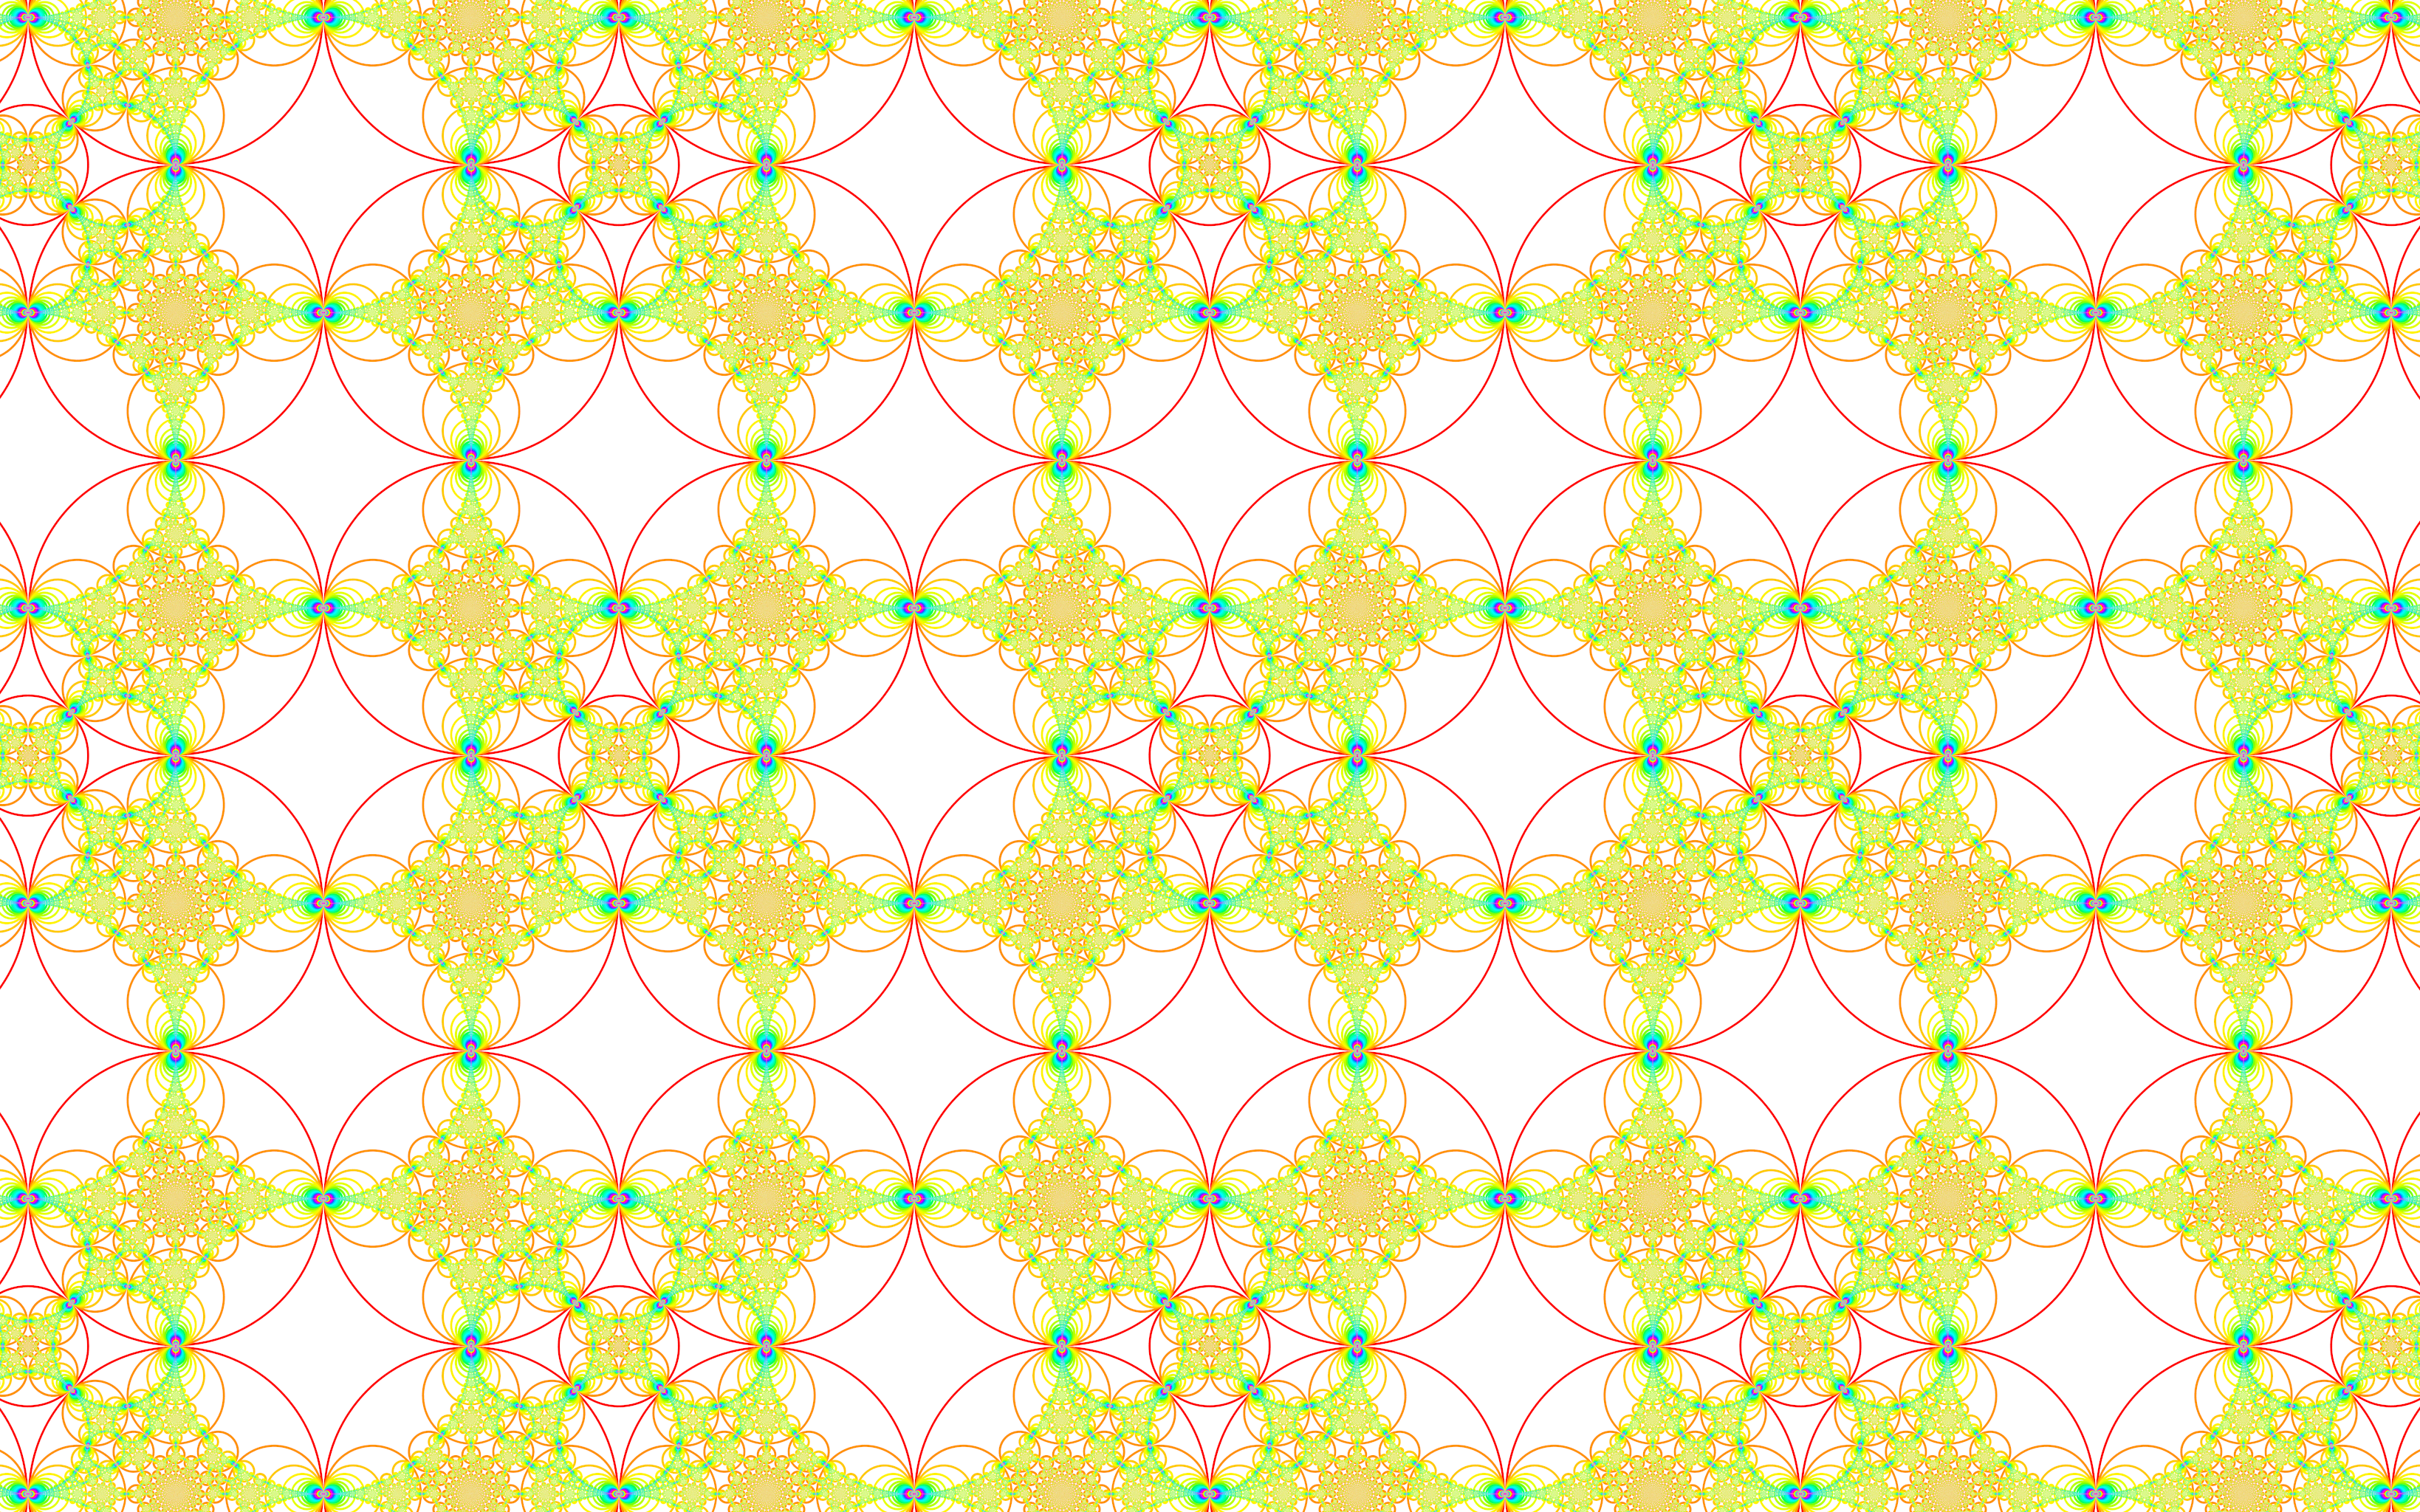
\includegraphics[height=1.35in, keepaspectratio]{img/application/edge/circleEdge.png}
  \caption{\textit{Edge of the circlte inversion fractal}}
  \label{fig:circleEdge}
 \hspace*{\fill}
\end{figure}

We can draw only edges of disks in circle inversion fractals.
We can estimate the distance from the center of the disks using jacobian
of circle inversions.

%% ヤコビアンを累積させていき,最後の円周からの距離を累積させたヤコビア
%% ンで割ることで,円周から点までの距離を得ることができる.

\subsection{Geometrical Representation of M\"obius Transformation Groups}

%% メビウス変換を円や球の反転で定義することによって,より直観的に生成元
%% を得て描画することができる.

In this paper, we mainly use circle or sphere inversions.
We can compose M\"obius transformations by even number of
inversion.
So far, we only use simple circle or sphere inversions.
Other interesting images can be generated using more
complicated M\"obius transformations.
It is known that we can construct any M\"obius transformation out of
inversions.
Thus, we can apply IIS to visualize fractals combining circle inversion
fractals and M\"obius transformation groups.
Moreover, we can tweak parameters of M\"obius transformations by
arranging geometrical objects like circles or lines on the plane.

\subsubsection{Two Dimensionanl Generators}

\begin{figure}[htbp]
 \begin{minipage}[t]{0.5\hsize}
  \begin{minipage}{0.25\hsize}
   \center
   \includegraphics[ height=1.4in, keepaspectratio]{./img/application/2dGen/infInvEdgedGen.pdf}
   \subcaption{\textit{Generator}}
   \label{fig:infCircleGen}
  \end{minipage}
  \hspace*{\fill}
  \begin{minipage}{0.25\hsize}
   \center
   \includegraphics[ height=1.4in, keepaspectratio]{./img/application/2dGen/infInvEdgedOrb.pdf}
   \subcaption{\textit{Orbit}}
   \label{fig:infCircleOrb}
  \end{minipage}
  \hspace*{\fill}
  \caption{\textit{Inversion in the circle with \\ infinite radius and
  four Schottky disks}}
  \label{fig:infCircle}
 \end{minipage}
 \begin{minipage}[t]{0.5\hsize}
  \begin{minipage}{0.25\hsize}
   \center
   \includegraphics[ height=1.4in, keepaspectratio]{./img/application/2dGen/translationEdgedGen.pdf}
   \subcaption{\textit{Generator}}
   \label{fig:translation2dGen}
  \end{minipage}
  \hspace*{\fill}
  \begin{minipage}{0.25\hsize}
   \center
   \includegraphics[ height=1.4in, keepaspectratio]{./img/application/2dGen/translationEdgedOrb.pdf}
   \subcaption{\textit{Orbit}}
   \label{fig:translation2dOrb}
  \end{minipage}
  \hspace*{\fill}
  \caption{\textit{Parallel translation generator and four Schottky disks}}
  \label{fig:translation2d}
 \end{minipage}
 \end{figure}

\begin{figure}[htbp]
 \begin{minipage}{0.5\hsize}
  \begin{minipage}{0.25\hsize}
   \center
   \includegraphics[ height=1.4in, keepaspectratio]{./img/application/2dGen/rotationEdgedGen.pdf}
   \subcaption{\textit{Generator}}
   \label{fig:rotation2dGen}
  \end{minipage}
 \hspace*{\fill}
  \begin{minipage}{0.25\hsize}
   \center
   \includegraphics[ height=1.4in, keepaspectratio]{./img/application/2dGen/rotationEdgedOrb.pdf}
   \subcaption{\textit{Orbit}}
   \label{fig:rotation2dOrb}
  \end{minipage}
  \hspace*{\fill}
  \caption{\textit{Rotation generator and three Schottky disks}}
  \label{fig:Rotation2d}
 \end{minipage}
 \begin{minipage}{0.5\hsize}
  \begin{minipage}{0.25\hsize}
   \center
   \includegraphics[ height=1.4in, keepaspectratio]{./img/application/2dGen/hyperbolicRect0.pdf}
   \subcaption{\textit{Generator}}
   \label{fig:hyperbolic2dGen}
  \end{minipage}
 \hspace*{\fill}
  \begin{minipage}{0.25\hsize}
   \center
   \includegraphics[ height=1.4in, keepaspectratio]{./img/application/2dGen/hyperbolicRect.pdf}
   \subcaption{\textit{Orbit}}
   \label{fig:hyperbolic2dOrb}
  \end{minipage}
 \hspace*{\fill}
  \caption{\textit{Hyperbolic generator and a Schottky disk}}
  \label{}
 \end{minipage}
\end{figure}

\begin{figure}[htbp]
 \begin{minipage}[t]{0.5\hsize}
  \begin{minipage}{0.25\hsize}
   \center
   \includegraphics[ height=1.4in, keepaspectratio]{./img/application/2dGen/parabolicRect0.pdf}
   \subcaption{\textit{Generator}}
   \label{fig:parabolic2dGen}
  \end{minipage}
 \hspace*{\fill}
  \begin{minipage}{0.25\hsize}
   \center
   \includegraphics[ height=1.4in, keepaspectratio]{./img/application/2dGen/parabolicRect.pdf}
   \subcaption{\textit{Orbit}}
   \label{fig:parabolic2dOrb}
  \end{minipage}
  \hspace*{\fill}
  \caption{\textit{The orbit of Parabolic generator and \\a Schottky disk}}
  \label{fig:parabolic2d}
 \end{minipage}
 \begin{minipage}[t]{0.5\hsize}
  \begin{minipage}{0.25\hsize}
   \center
   \includegraphics[ height=1.4in, keepaspectratio]{./img/application/2dGen/loxo0.pdf}
   \subcaption{\textit{Generator}}
   \label{fig:loxo2dGen}
  \end{minipage}
 \hspace*{\fill}
  \begin{minipage}{0.25\hsize}
   \center
   \includegraphics[ height=1.4in, keepaspectratio]{./img/application/2dGen/loxoOrb.pdf}
   \subcaption{\textit{Orbit}}
   \label{fig:loxo2dOrb}
  \end{minipage}
 \hspace*{\fill}
  \caption{\textit{Loxodromic generator and a Schottky disk}}
  \label{fig:loxodromic2d}
 \end{minipage}
\end{figure}

\noindent\textbf{Inversion in a Circle with Infinite Radius.}
An inversion in a circle with infinite radius is treated as a reflection
over a border line of half plane. See Figure
\ref{fig:infCircle}\subref{fig:infCircleGen}.
The four inversion circles are lying on the right side, and there is the
orange region on the left side. The region is is a half plane, that is, a
disk with infinite radius. Its boundary is colored with white line.
The orbit is shown in
Figure \ref{fig:infCircle}\subref{fig:infCircleOrb}.
As we can see, the circles are reflected over the white line.

\noindent\textbf{Parallel Translation.}
A composition of reflections over two parallel half planes facing each
other generates a parallel translation. See Figure
\ref{fig:translation2d}\subref{fig:translation2dGen}.
There are two orange half planes on the right and left sides.
The orbit is shown in Figure
\ref{fig:translation2d}\subref{fig:translation2dOrb}.

\noindent\textbf{Rotation.}
A composition of reflections over two crossing half planes generates a
rotation. The generator is shown in Figure
\ref{fig:Rotation2d}\subref{rotation2dGen}
The two half planes are crossing. The rotation axis is crossing point of
white border lines. The orbit is shown in Figure 
\ref{fig:Rotation2d}\subref{rotation2dOrb}.
It has a rotation symmetry and it is an elliptic transformation.

\noindent\textbf{Composition of Two Circles.}
%% Hyperbolic, parabolic, elliptic

\noindent\textbf{Loxodromic.}


\subsubsection{Three Dimensionanl Generators}

\begin{figure}[h!tbp]
 \begin{minipage}[t]{0.5\hsize}
  \begin{minipage}{0.25\hsize}
   \center
   \includegraphics[width=1.4in, height=1.4in, keepaspectratio]{./img/application/3dGen/infSphereGen.pdf}
   \subcaption{\textit{Generator}}
   \label{fig:infSphereGen}
  \end{minipage}
  \hspace*{\fill}
  \begin{minipage}{0.25\hsize}
   \center
   \includegraphics[width=1.4in, height=1.4in, keepaspectratio]{./img/application/3dGen/infSphereOrbit.pdf}
   \subcaption{\textit{Orbit}}
   \label{fig:infSphereOrb}
  \end{minipage}
  \hspace*{\fill}
  \caption{\textit{Inversion in the sphere with infinite radius, four
  Schottky spheres, and a base sphere}}
  \label{fig:infSphere}
 \end{minipage}
 \hspace*{\fill}
 \begin{minipage}[t]{0.5\hsize}
  \begin{minipage}{0.25\hsize}
   \center
   \includegraphics[width=1.4in, height=1.4in, keepaspectratio]{./img/application/3dGen/translationGen.pdf}
   \subcaption{\textit{Generator}}
   \label{fig:translation3dGen}
  \end{minipage}
  \hspace*{\fill}
 \begin{minipage}{0.25\hsize}
  \center
  \includegraphics[width=1.4in, height=1.4in, keepaspectratio]{./img/application/3dGen/translationOrbit.pdf}
  \subcaption{\textit{Orbit}}
    \label{fig:translation3dOrb}
 \end{minipage}
  \hspace*{\fill}
  \caption{\textit{Parallel translation generator, six Schottky spheres
  and a base sphere}}
  \label{fig:translation3d}
 \end{minipage}
\end{figure}

\begin{figure}[h!tbp]
 \begin{minipage}[t]{0.5\hsize}
  \begin{minipage}{0.25\hsize}
   \center
    \includegraphics[width=1.4in, height=1.4in, keepaspectratio]{./img/application/3dGen/compParabolicGen.pdf}
    \subcaption{\textit{Generator}}
    \label{fig:compParabolicGen}
  \end{minipage}
  \hspace*{\fill}
  \begin{minipage}{0.25\hsize}
   \center
   \includegraphics[width=1.4in, height=1.4in, keepaspectratio]{./img/application/3dGen/compParabolicOrb.pdf}
   \subcaption{\textit{Orbit}}
   \label{fig:compParabolicOrb}
  \end{minipage}
  \hspace*{\fill}
  \caption{\textit{Compound parabolic generator, six \\Schottky spheres
  and a base sphere}}
  \label{fig:compParabolic}
 \end{minipage}
 \hspace*{\fill}
 \begin{minipage}[t]{0.5\hsize}
  \begin{minipage}{0.25\hsize}
   \center
   \includegraphics[width=1.4in, height=1.4in, keepaspectratio]{./img/application/3dGen/rotationGen.pdf}
   \subcaption{\textit{Generator}}
   \label{fig:rotationGen}
  \end{minipage}
  \hspace*{\fill}
  \begin{minipage}{0.25\hsize}
   \center
   \includegraphics[width=1.4in, height=1.4in, keepaspectratio]{./img/application/3dGen/rotationOrb.pdf}
   \subcaption{\textit{Orbit}}
   \label{fig:rotationOrb}
  \end{minipage}
  \hspace*{\fill}
  \caption{\textit{Rotation generator, four Schottky spheres, and a base
  sphere}}
  \label{fig:rotation3d}
 \end{minipage}
\end{figure}

\begin{figure}[h!tbp]
 \begin{minipage}{0.5\hsize}
  \begin{minipage}{0.25\hsize}
   \center
   \includegraphics[width=1.4in, height=1.4in, keepaspectratio]{./img/application/3dGen/loxoGenSimple.pdf}
   \subcaption{\textit{Generator}}
   \label{fig:loxoGen3d}
  \end{minipage}
  \hspace*{\fill}
  \begin{minipage}{0.25\hsize}
   \center
   \includegraphics[width=1.4in, height=1.4in, keepaspectratio]{./img/application/3dGen/loxoOrbSimple.pdf}
   \subcaption{\textit{Orbit}}
   \label{fig:loxoOrb3d}
  \end{minipage}
  \hspace*{\fill}
 \caption{\textit{Hyperbolic generator and a base sphere}}
  \label{fig:loxo3d}
 \end{minipage}
 \hspace*{\fill}
 \begin{minipage}{0.5\hsize}
  \begin{minipage}{0.25\hsize}
   \center
   \includegraphics[width=1.4in, height=1.4in, keepaspectratio]{./img/application/3dGen/parabolicOneGen.pdf}
   \subcaption{\textit{Generator}}
   \label{fig:parabolic3dGen}
  \end{minipage}
  \hspace*{\fill}
  \begin{minipage}{0.25\hsize}
   \center
   \includegraphics[width=1.4in, height=1.4in, keepaspectratio]{./img/application/3dGen/parabolicOneOrb.pdf}
  \subcaption{\textit{Orbit}}
   \label{fig:parabolic3dOrb}
  \end{minipage}
  \hspace*{\fill}
  \caption{\textit{Parabolic generator and a base sphere}}
  \label{fig:parabolic3d}
 \end{minipage}
\end{figure}

\begin{figure}[h!tbp]
 \begin{minipage}[t]{0.5\hsize}
  \begin{minipage}[t]{0.25\hsize}
   \center
   \includegraphics[width=1.4in, height=1.4in, keepaspectratio]{./img/application/3dGen/loxoOrbSch.pdf}
   \subcaption{\textit{Hyperbolic}}
  \end{minipage}
  \hspace*{\fill}
  \begin{minipage}[t]{0.25\hsize}
   \center
   \includegraphics[width=1.4in, height=1.4in, keepaspectratio]{./img/application/3dGen/parabolicOrb.pdf}
   \subcaption{\textit{Parabolic}}
  \end{minipage}
  \hspace*{\fill}
  \caption{\textit{The orbit generated by a composition \\of two spheres and six Schottky
  spheres}}
  \label{fig:complicated3d}
 \end{minipage}
 \hspace*{\fill}
 \begin{minipage}[t]{0.5\hsize}
  \begin{minipage}[t]{0.25\hsize}
   \center
   \includegraphics[width=1.4in, height=1.4in, keepaspectratio]{./img/application/3dGen/compLoxoOneGen.pdf}
   \subcaption{\textit{Generator}}
   \label{fig:compLoxoGen}
  \end{minipage}
 \hspace*{\fill}
  \begin{minipage}[t]{0.25\hsize}
   \center
   \includegraphics[width=1.4in, height=1.4in, keepaspectratio]{./img/application/3dGen/compLoxoOneOrb.pdf}
   \subcaption{\textit{Orbit}}
   \label{fig:compLoxoOrb}
  \end{minipage}
  \hspace*{\fill}
  \caption{\textit{Compound loxodromic generator and a base sphere}}
  \label{fig:compLoxo}
 \end{minipage}
\end{figure}

\noindent\textbf{Inversion in a Sphere with Infinite Radius.}

\noindent\textbf{Parallel
Translation~\footnote{\url{https://www.shadertoy.com/view/lsjyzK}}.}

\noindent\textbf{Rotation.}

\noindent\textbf{Composition of Two
Spheres~\footnote{\url{https://www.shadertoy.com/view/ldByDW}}.}
%% Hyperbolic, parabolic, elliptic

\noindent\textbf{Compound Loxodromic~\footnote{\url{https://www.shadertoy.com/view/MdjyRV}}.}

\subsection{Sphairahedra and Three-dimensional Fractals}

%% 球面体のタイリングもIISで描画することができる

In 2003, Kazushi Ahara and Yoshiaki Araki invented
\textit{Sphairahedron} to introduce new kind of three dimensional
fractals \cite{ahara2003sphairahedral}.

Sphairahedron is coined word combining two words sphaira- and -hedron.

The fractals are generated by tiling of sphairahedra.

We use IIS for three dimensional tiling.
This method uses 
For more details, read \cite{bridges2018:171}

%#!uplatex main.tex

\section{Conclusion}

In this paper, we introduced an efficient algorithm
called Iterated Inversion System (IIS) to visualize Kleinian
groups based on circle inversions and sphere inversions.

IIS has a constraint that we have to compute in parallel;
Nevertheless it is useful. The application range of IIS is broad.
We can render many images related to Kleinian groups and tiling using
IIS.

There is a fractal called \textit{pseudo-kleinian} and
there are algorithms related to pseudo-kleinian.
The algorithms are fast like IIS, but they are not a Kleinian group which
mathematician means.
However, IIS and mathematics are developed close
together.
Therefore IIS is took notice by researcher who study Kleinian groups as
pure mathematics and computer graphics.

On the other hand, there are also Kleinian groups, which we can not
visualize using IIS.
Our final goal is that for all Kleinian groups, we develop this kind of
efficient algorithm and get mathematical results from obtained images.


\addcontentsline{toc}{section}{References}
\printbibliography

\end{document}
